\documentclass[10pt]{beamer}

%\usetheme{metropolis}
%\usetheme{AnnArbor}
\usetheme[progressbar=frametitle]{metropolis}
%\usecolortheme{beaver}
\usepackage{appendixnumberbeamer}

\usepackage{booktabs}
\usepackage[scale=2]{ccicons}

\usepackage{pgfplots}
\usepgfplotslibrary{dateplot}

\usepackage{xspace}
\newcommand{\themename}{\textbf{\textsc{metropolis}}\xspace}
%\usepackage[brazil]{babel}  % AAB
\usepackage{bibentry}       % AAB
\usepackage{amsmath, bm}    % AAB
\usepackage{tikz}           % AAB    
\usetikzlibrary{shapes,arrows,shadows}  % AAB inserido
%\usepackage[utf8]{inputenc}                  % AAB inserido
                                              % AAB inserido
\usepackage[caption=false,font=normalsize,labelfont=sf,textfont=sf]{subfig}
%\usepackage[caption=false,font=footnotesize]{subfig}
%
\DeclareMathOperator{\traco}{tr} %AAB
\graphicspath{{../Dissertacao/figuras/}}        % AAB - caminho das figuras
%\graphicspath{{../Images/PDF/}}                 % AAB - caminho das figuras (recomendável) 

\title{Fusion of Evidences for Edge Detection in PolSAR Images}
%\subtitle{A modern beamer theme}
\date{\today}
\author{Anderson Adaime de Borba - Mackenzie-BR - IBMEC-SP\\
        Dr. Mauricio Marengoni - Mackenzie-BR\\
        Dr. Alejandro Frery - UFAL-BR} 
\institute{IBMEC-SP - 2019}
\titlegraphic{\hfill
\includegraphics[height=1.1cm]{logo_mack1.pdf}}
\titlegraphic{\hfill
\includegraphics[height=1.1cm]{laccan_ufal.pdf}}
\titlegraphic{\hfill
\includegraphics[height=1.1cm]{logo_ibmec1.pdf}}

\titlegraphic{%
      
\includegraphics[width=.2\textwidth]{laccan_ufal.pdf}\hfill
     % 
\includegraphics[width=3cm,height=1.6cm]{ufal.pdf}\hfill
      
\includegraphics[width=.2\textwidth]{logo_mack1.pdf}
      
\includegraphics[width=.4\textwidth]{logo_ibmec1.pdf}
   }

\begin{document}

\maketitle

\begin{frame}[fragile]{PolSAR Image}
\begin{alertblock}{PolSAR important characteristics}
\begin{itemize}
\item[-] can be on raised platforms, crewed aircraft or not, satellites orbiting the  earth or other planets;
\item[-] it is a viable and practical imaging technique;
\item[-] PolSAR images has a high resolution;
\item[-] synthesizes long antenna openings;
\item[-] radars produce images day and night;
\item[-] climate does not interfere in image capture.
\item[-] SAR imaging systems operate in the microwave region of the electromagnetic spectrum, usually between the P-band - and the K-band.
\end{itemize}
\end{alertblock}
\end{frame}
%
\begin{frame}[fragile]{PolSAR Image}
\begin{alertblock}{Economy Applications}
\begin{itemize}
\item[-] \href{http://www.h2020-eoxposure.eu/}{\alert{EOxposure-} Project with European Union} ;
\item[-] He goal of the EOxposure project is to build tools to quantify the exposure of population and economic assets to multiple risks using novel information layers from current and future Earth Observation (EO) missions, as well as the growing sensor web on the ground;
\item[-] Housing condition mapping;
\item[-] Disease spread proxies;
\item[-] Physical proxies to security threats. 
\end{itemize}
\end{alertblock}
\end{frame}
\begin{frame}[fragile]{PolSAR Image}
\begin{alertblock}{Economy Applications - The Gross Domestic Product - GDP}
\begin{itemize}
\item[-] \href{https://www.sciencedirect.com/science/article/pii/S0165176518304452}{Article adress};
\item[-] We estimate a TVP VAR via maximum likelihood;
\item[-] The stochastic volatility of the system is modeled via a Wishart process.
\item[-] The law of motion of VAR coefficients allows for multivariate stochastic volatility;
\item[-] The likelihood function of this model and all filtering formulas for tracking the latent states are obtained in closed form.
\end{itemize}
\end{alertblock}
\end{frame}

\begin{frame}[fragile]{PolSAR Image}
\begin{alertblock}{Economy Applications - The View from Above: Applications of Satellite Data in Economics}
\begin{itemize}
\item[-] \href{http://dave-donaldson.com/wp-content/uploads/2016/10/Donaldson_Storeygard_JEP.pdf}{Article adress};
\item[-] Forest Cover over Time in Riau Province, Indonesia;
\item[-] Aerosol Index of Particulate Air Pollution in Indonesia during Massive Wildfires in 1997;
\item[-] Roofs in Kibera, Nairobi;
\end{itemize}
\end{alertblock}
\end{frame}

\begin{frame}[fragile]{PolSAR Image}
\begin{figure}[hbt]
	\centering
	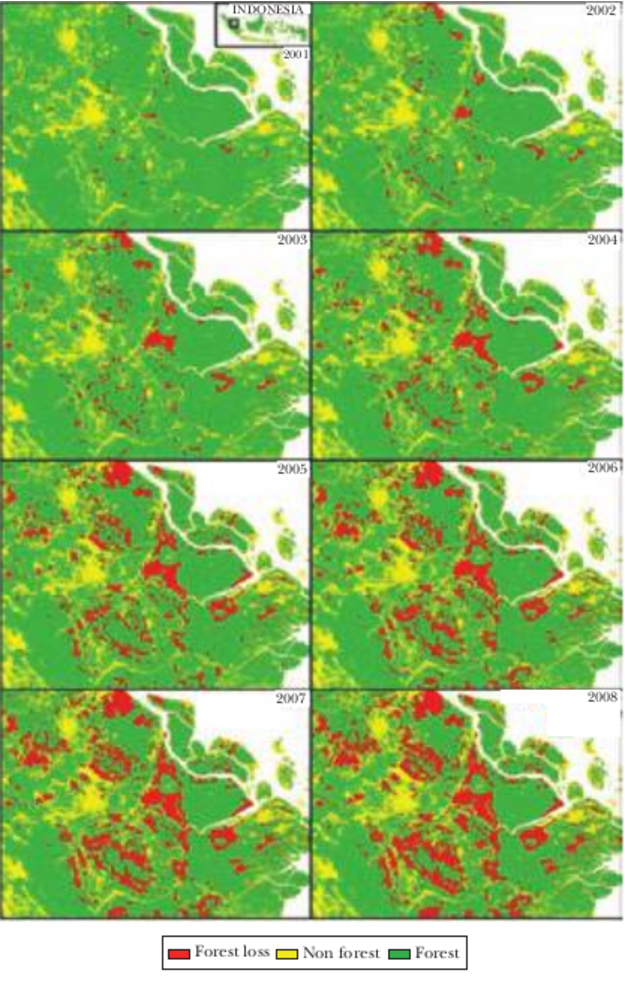
\includegraphics[width=.4\linewidth]{econ1_crop}%
	\caption{Forest Cover over Time in Riau Province, Ref.~\cite{ds}}
\label{fig4}
\end{figure}
\end{frame}

\begin{frame}[fragile]{PolSAR Image}
\begin{figure}[hbt]
	\centering
	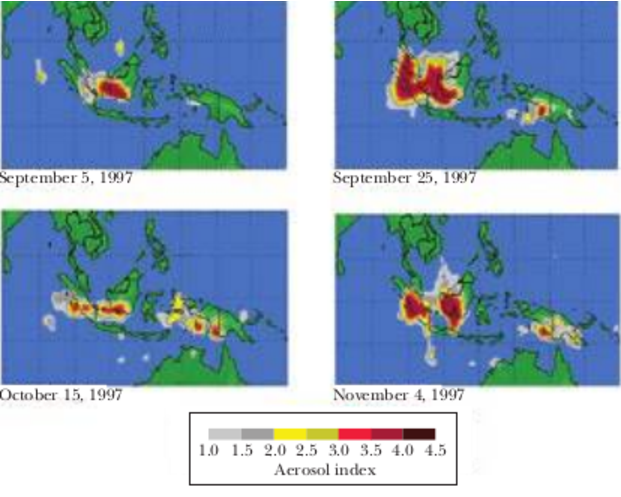
\includegraphics[width=.6\linewidth]{econ2_crop}%
	\caption{Aerosol Index of Particulate Air Pollution in Indonesia, Ref.~\cite{ds}}
\label{fig4}
\end{figure}
\end{frame}

\begin{frame}[fragile]{PolSAR Image}
\begin{figure}[hbt]
	\centering
	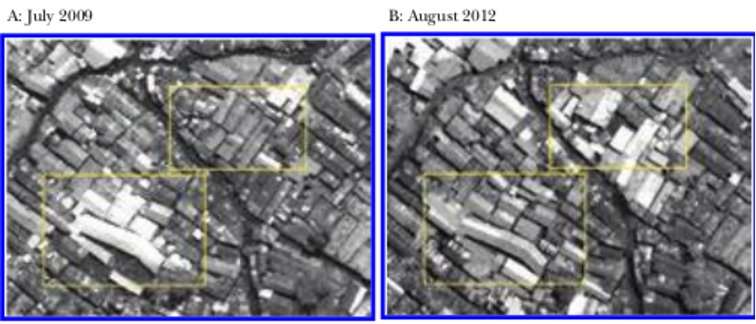
\includegraphics[width=.6\linewidth]{econ3_crop}%
	\caption{Roofs in Kibera, Nairobi, Ref.~\cite{ds}}
\label{fig4}
\end{figure}
\end{frame}

\begin{frame}[fragile]{Statistical Modeling}
\begin{alertblock}{Statistical modeling for PolSAR data (1 - Look)}
\begin{itemize}
\item The complex scattering matrix $\mathbf{S}$:
\begin{equation}
\mathbf{S} = \left[
\begin{array}{cc}
	S_\text{hh}   & S_\text{hv}   \\
	S_\text{vv}   & S_\text{vv}   
\end{array}
\right].
\end{equation}\label{eq_01}
\item The medium of propagation of waves is reciprocal
$$\mathbf{s}=[S_\text{hh},S_\text{hv},S_{\text{vv}}]^T.$$
\end{itemize}
\end{alertblock}
\end{frame}

\begin{frame}[fragile]{Statistical Modeling}
\begin{alertblock}{Statistical modeling for PolSAR data (1 - Look)}
\begin{itemize}
\item The probability density function (pdf):
\begin{equation}
    f_{\mathbf{s}}(\mathbf{s};\Sigma)=\frac{1}{\pi^3|\Sigma|} \exp(-\mathbf{s}^H\Sigma^{-1}\mathbf{s}),
    \label{eq_02}
\end{equation}
        \begin{description}
        \item[-] $|\cdot|$ is the determinant, 
        \item[-] $H$ denotes the conjugate complex number, 
        \item[-] $\Sigma$ is the covariance matrix of $\mathbf{s}$ such that $\Sigma=E[\mathbf{ss}^H]$,
        \item[-] $E[\cdot]$ denotes the expected value. 
        \item[-] The distribution of $\mathbf{s}$ is assumed to be  Gaussian circular complex multivariate with zero mean $N^{C}_3(0,\Sigma)$.
        \end{description}
\end{itemize}
\end{alertblock}
\end{frame}
%
\begin{frame}[fragile]{Statistical Modeling}
\begin{alertblock}{Statistical modeling for PolSAR data (L - Looks)}
\begin{itemize}
\item The estimated sample covariance matrix:
\begin{equation}
    \mathbf{Z}=\frac{1}{L}\sum_{\ell=1}^{L} {\mathbf{s}_\ell}{\mathbf{s}_\ell}^H,
    \label{eq_03}
\end{equation}
\begin{description}
      \item[-] $\mathbf{s}_\ell$, $\ell = 1, \dots, L$;
      \item[-] $L$ independent samples of complex vectors distributed as $\mathbf{s}$. 
\end{description}
\end{itemize}
\end{alertblock}
\end{frame}

\begin{frame}[fragile]{Statistical Modeling}
\begin{alertblock}{Statistical modeling for PolSAR data (L - Looks)}
\begin{itemize}
\item Multilooked Wishart distribution with probability density function:
\begin{equation}
    f_{\mathbf{Z}}(\mathbf{Z};\Sigma_{s},L)=\frac{L^{mL}|\mathbf{Z}|^{L-m}}{|\Sigma_{s}|^{L}\Gamma_m(L)} \exp(-L\traco(\Sigma_{s}^{-1}\mathbf{Z})),
    \label{eq_04}
\end{equation} 
\begin{description}
\item[-] $\traco(\cdot)$ is the trace operator,
\item[-] $\Gamma_m(L)$ is a multivariate Gamma function
\begin{equation*}
	\Gamma_m(L)=\pi^{\frac{1}{2}m(m-1)} \prod_{i=0}^{m-1}\Gamma(L-i),
\end{equation*}
\item[-]$\Gamma(\cdot)$ is the Gamma function,
\item[-]$m=3$,
\item[-]$\mathbf{Z}\sim W(\Sigma, L)$, 
%\item[-]$E[\mathbf{Z}]=\Sigma$. 
\end{description} 
\end{itemize}
\end{alertblock}
\end{frame}

\begin{frame}[fragile]{Edges detection}
\begin{alertblock}{Method}
The following procedure is proposed to detected edges in the $\text{hh}$, $\text{hv}$ and $\text{vv}$ channels:
\begin{itemize}
	\item identify the centroid of a region of interest (ROI) in an automatic, semi-automatic or manual manner;
	\item cast rays from the centroid to the outside of the area;
	\item collect data around the rays using the  Bresenham's midpoint line algorithm, ideally the size of a pixel;
	\item detect points in the data strips which provide evidence of changes in their statistical properties, i.e., a transition point that defines edge evidence;
	\item use the Generalized Simulated Annealing (GenSA) method, Ref.~\cite{xgsh}, to find maximum points in the functions of interest;
	\item fuse the evidence of detected edges in the $\text{hh}$, $\text{hv}$ and $\text{vv}$ channels.
\end{itemize}
\end{alertblock}
\end{frame}

\begin{frame}[fragile]{Edges detection}
\begin{alertblock}{ROI Flevoland Example} 
\begin{figure}[hbt]
\centering
	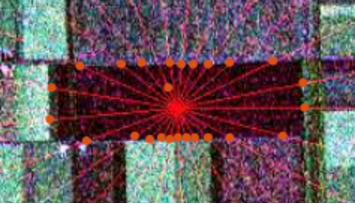
\includegraphics[width=.7\linewidth]{flevoland_radial_25_point_hh_crop}
	\caption{Edges detection example ($\text{hh}$ channel).}
\label{fig1}
\end{figure}
\end{alertblock}
\end{frame}

\begin{frame}[fragile]{PolSAR Image}
\begin{alertblock}{Maximum Likelihood Estimator (MLE)}
\begin{itemize}
	\item Suppose $\mathbf{X}=(X_1,X_2,\dots,X_n)^T$ is a random vector distributed according to the probability density function $f(\mathbf{x},\mathbf{\theta})$ with parameters $\mathbf{\theta}=(\theta_1,\dots,\theta_d)^T$ in the parameter space $\Theta$.
    \item The likelihood function is
\begin{equation*}
   L(\theta;\mathbf{X}) = \prod_{i=1}^{n}f(x_i;\theta),
\end{equation*}
   \item log-likelihood function is
\begin{equation}
	\ell(\theta;\mathbf{X})= \ln L(\theta;\mathbf{X}) = \sum_{i=1}^{n}\ln f(x_i;\theta),
	\label{eq_05}
\end{equation}
     \item $\widehat{\theta}= \arg\max\limits_{\theta\in\Theta}L(\theta;\mathbf{x})$,
     \item $\widehat{\theta}= \arg\max\limits_{\theta\in\Theta}\ell(\theta;\mathbf{x})$.
\end{itemize}
\end{alertblock}
\end{frame}

\begin{frame}[fragile]{Edges detection}
\begin{alertblock}{Maximum Likelihood Estimator (MLE) for two regions A and B}
\begin{itemize}
\item The estimates for the covariance matrices can be found using the maximum likelihood estimator denoted by $\widehat{\Sigma}$, Ref.~\cite{good}: 
\begin{equation}
\widehat{\Sigma_{I}}(j) = \left\{
\begin{array}{lc}
	j^{-1}\sum_{k=1}^{j}\mathbf{Z}_{k}  & \mbox{if}\quad I=A,  \\
        (N-j)^{-1}\sum_{k=j+1}^{N}\mathbf{Z}_{k} & \mbox{if}\quad I=B.
\end{array}
\right.\label{eq_08}
\end{equation}
	\item likelihood function
	 \begin{equation}
	L(j)=\prod_{k_1=1}^{j}f_{\mathbf{Z}}(\mathbf{Z}_{k_1};\widehat\Sigma_{A},L) \prod_{k_2=j+1}^{N}f_{\mathbf{Z}}(\mathbf{Z}_{k_2};\widehat\Sigma_{B},L),
	\label{eq_06}
\end{equation}
    \item log-likelihood function
\begin{equation}
\ell(j) =
	\sum_{k_1=1}^{j}\ln f_{\mathbf{Z}}(\mathbf{Z}_{k_1}; \widehat\Sigma_{A},L) + \sum_{k_2=j+1}^{N}\ln f_{\mathbf{Z}}(\mathbf{Z}_{k_2}; \widehat\Sigma_{B},L).
	\label{eq_07}
\end{equation}
\end{itemize}
\end{alertblock}
\end{frame}


\begin{frame}[fragile]{Edges detection}
\begin{alertblock}{Maximum Likelihood Estimator (MLE)}
\begin{itemize}
	\item After algebraic manipulations on each term of the summation, it is obtained:
\begin{align}\nonumber
	\ell(j)&=N\left[mL(\ln{L}-1)-\ln{\Gamma_m(L)}\right]\\\nonumber
	&- L\left[j\ln{|\widehat{\Sigma}_{A}(j)|} +(N-j)\ln{|\widehat{\Sigma}_{B}(j)|}\right] \\
	&+ (L-m)\sum_{k=1}^{N}\ln{|\mathbf{Z}_{k}|}.\label{eq_09}
\end{align}

\item The argument of the maximum $\widehat{\jmath}$ is the edge evidence that will be used in our fusion methods.
\end{itemize}
\end{alertblock}
\end{frame}

\begin{frame}[fragile]{Edges detection}
\begin{alertblock}{Application in simulated images}
	\begin{figure}[hbt]
     \subfloat[Pauli decomposition \label{fig2:a}]{%
       %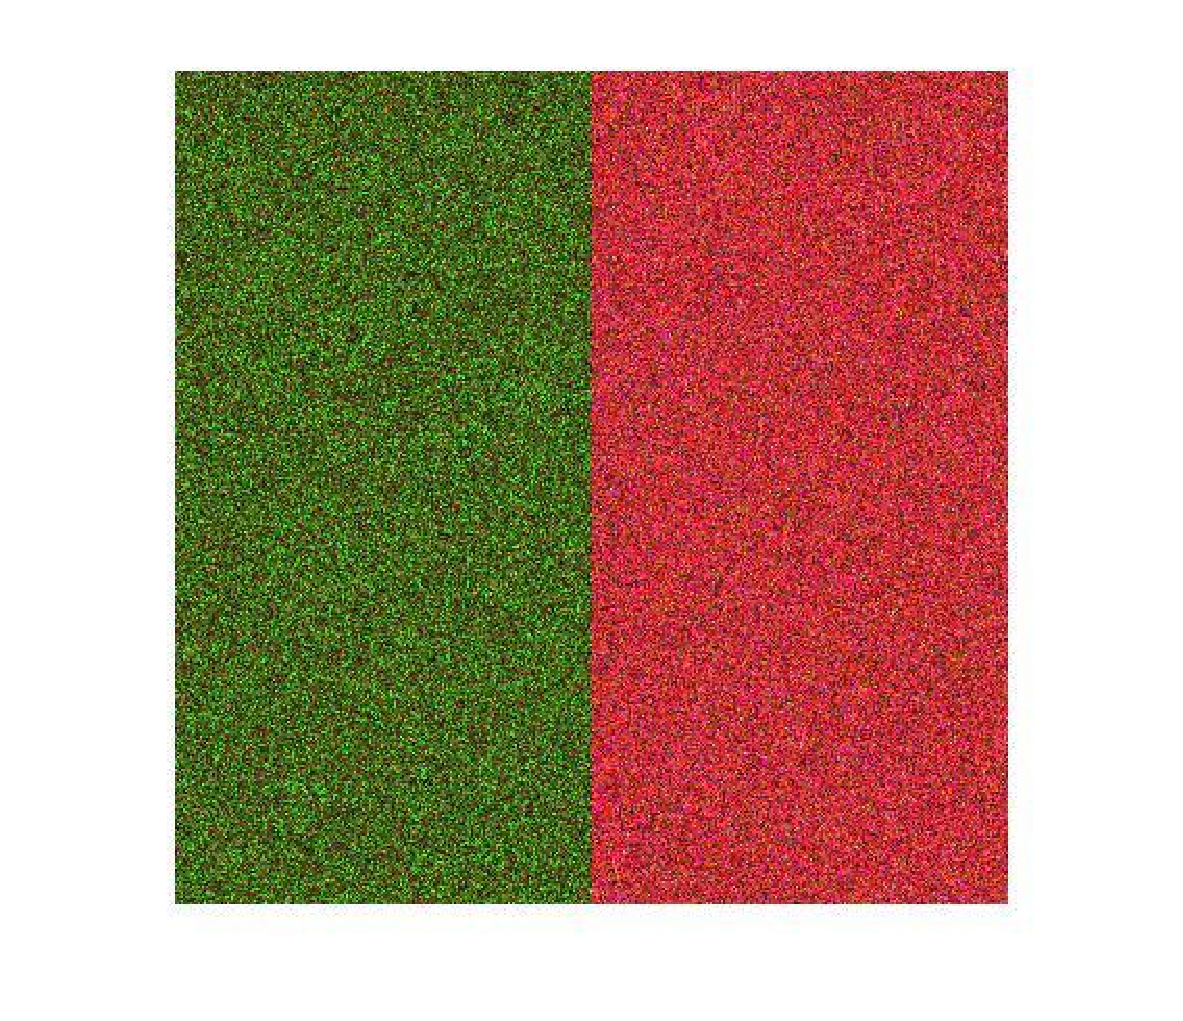
\includegraphics[viewport= 80 50 490 460, clip=true, width=0.23\textwidth]{phanton_nhfc_dec_pauli}}      
       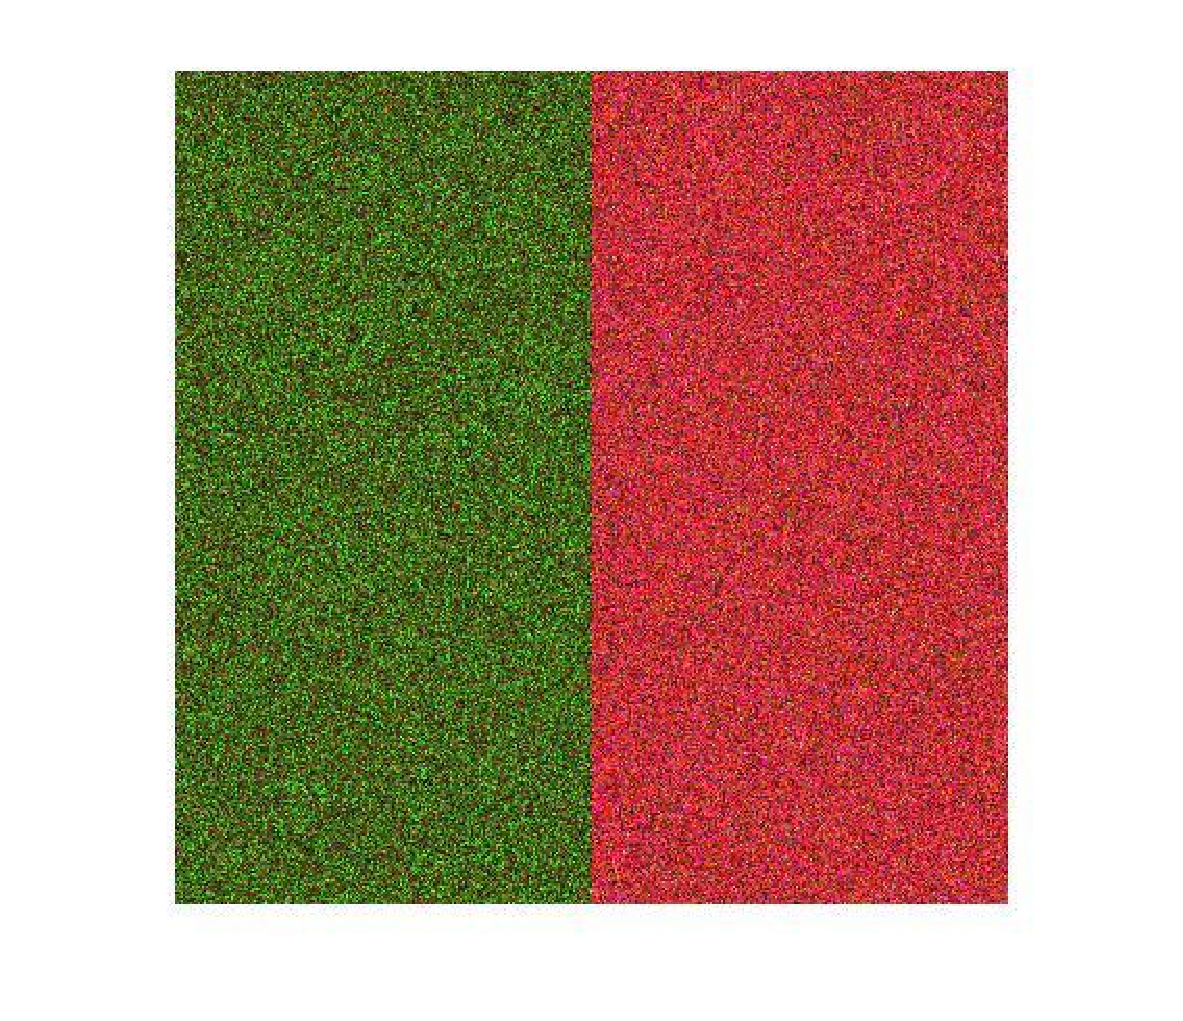
\includegraphics[viewport= 80 50 490 460, clip=true, width=0.45\textwidth]{phanton_nhfc_dec_pauli}}  
     \subfloat[Marginal densities of the $\text{hh}$ channel\label{fig2:b}]{%
       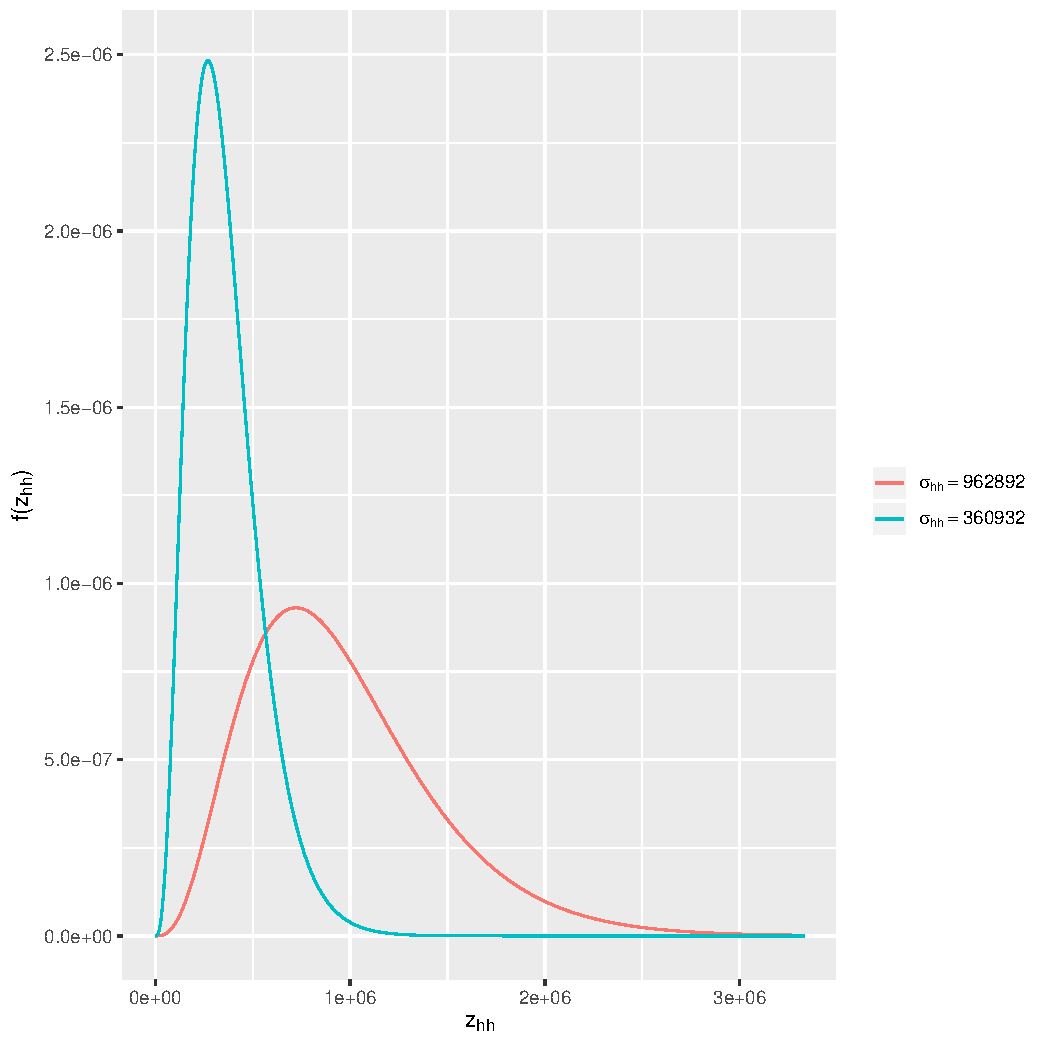
\includegraphics[width=0.45\textwidth]{grafico_pdf_nhfc_2014_sigma_hh_artigos}
     }
    \caption{Model and observations}
     \label{fig2}
\end{figure}
\end{alertblock}
\end{frame}
\begin{frame}[fragile]{Edges detection}
\begin{alertblock}{Application in simulated images}
	\begin{figure}[hbt]
	\centering
     \subfloat[Channel $\text{hh}$ \label{fig3:a}]{%
       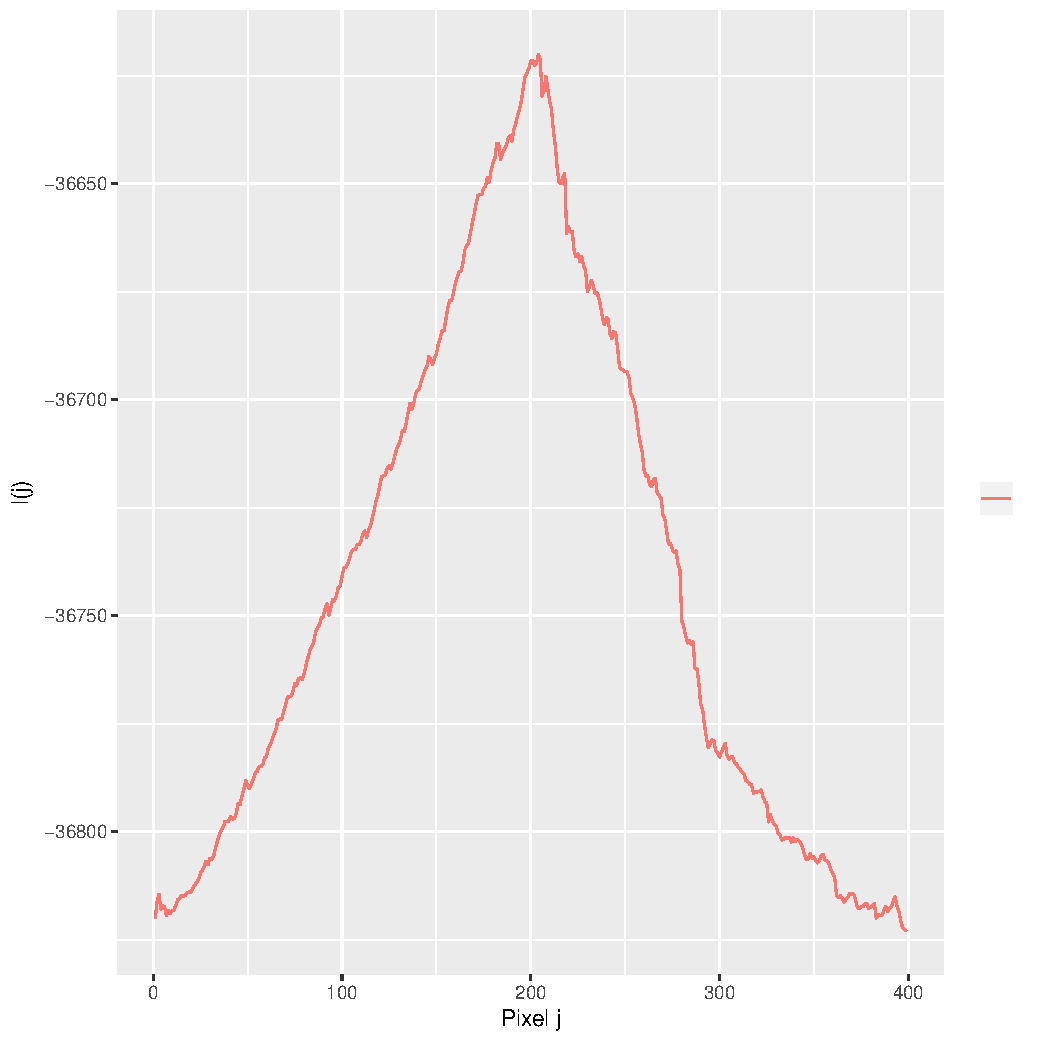
\includegraphics[width=0.32\linewidth]{grafico_l_nhfc_2014_sigmahh_artigos}}
     \subfloat[Channel $\text{hv}$ \label{fig3:b}]{%
       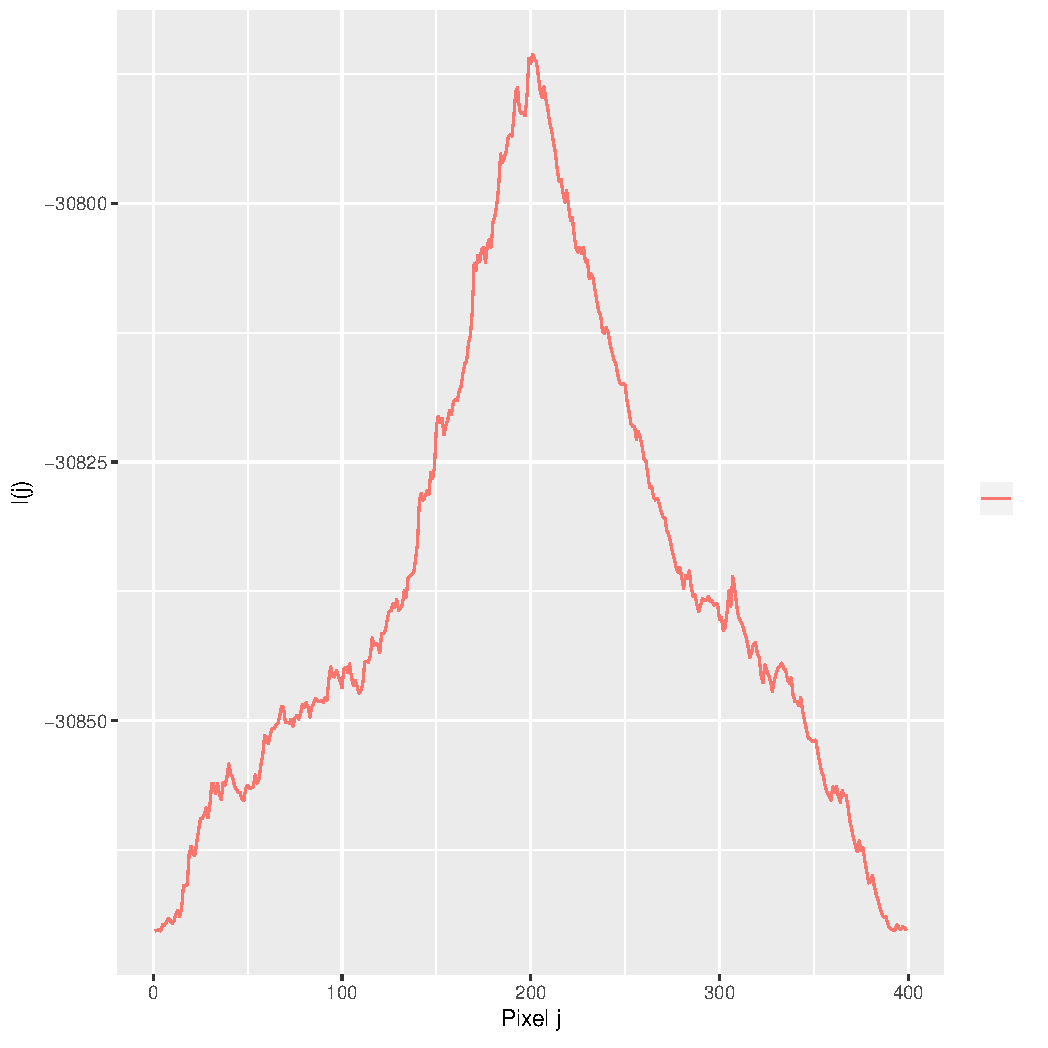
\includegraphics[width=0.32\linewidth]{grafico_l_nhfc_2014_sigmahv_artigos}}
     \subfloat[Channel $\text{vv}$ \label{fig3:c}]{%
       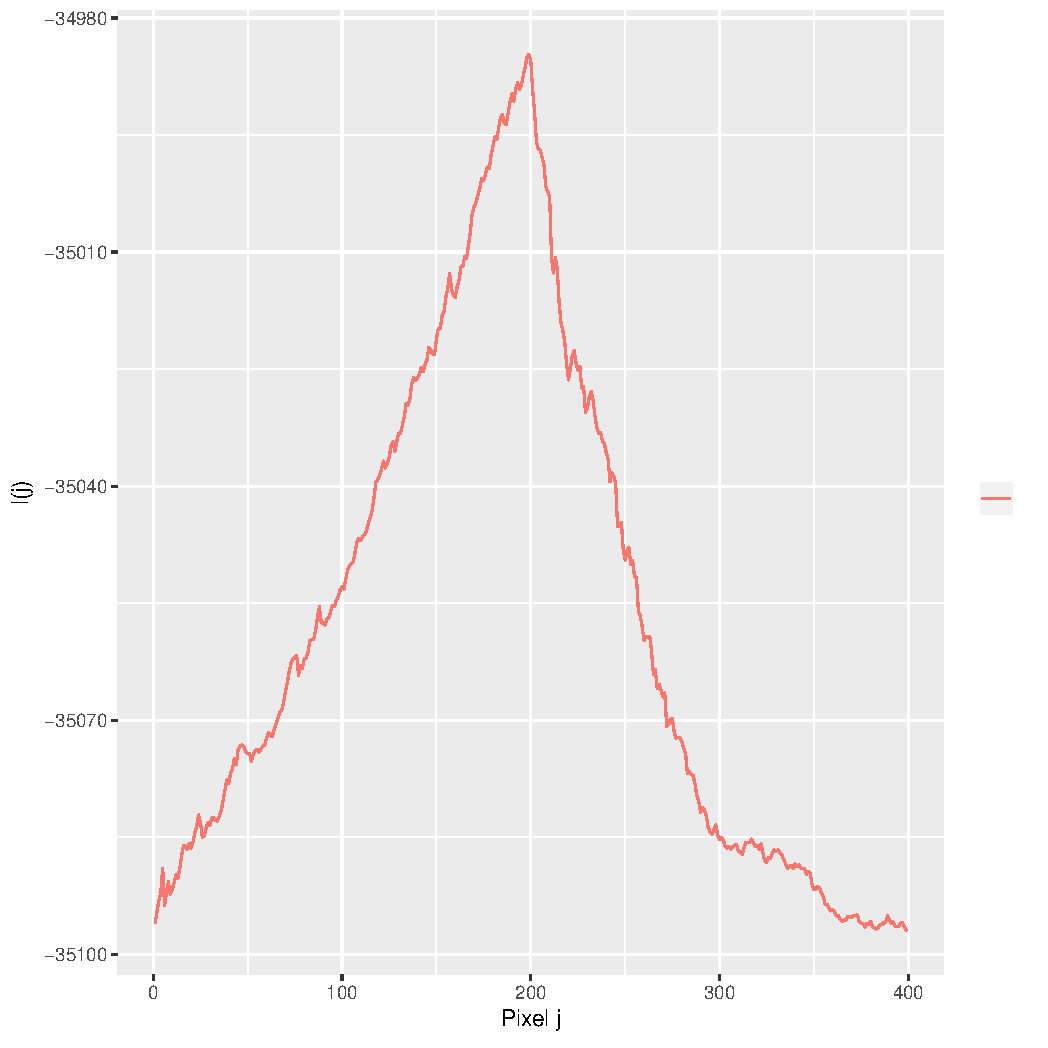
\includegraphics[width=0.32\linewidth]{grafico_l_nhfc_2014_sigmavv_artigos}}
     \caption{$l(j)$ log-likelihood function}
     \label{fig3}
   \end{figure}	
\end{alertblock}
\end{frame}


\begin{frame}[fragile]{Edges detection}
\begin{alertblock}{Application in simulated images} 
	\begin{figure}[hbt]
	\centering
	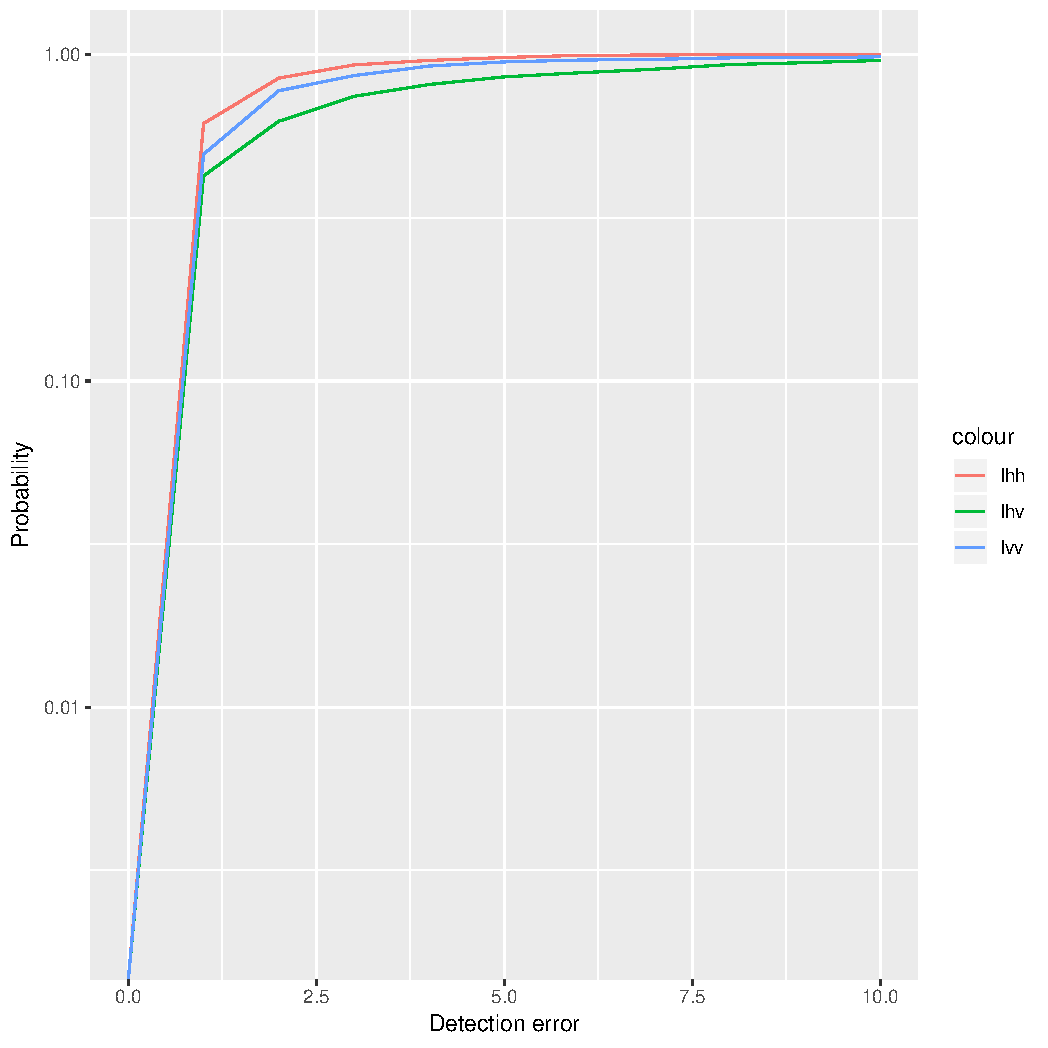
\includegraphics[width=.6\linewidth]{metricas_ihh_ivh_ivv_nhfc_artigos}%
	\caption{Probability of detecting edges evidences.}
\label{fig4}
\end{figure}
\end{alertblock}
\end{frame}

\begin{frame}[fragile]{Evidence Fusion}
\begin{alertblock}{Average Fusion}
\pgfdeclarelayer{background}
\pgfdeclarelayer{foreground}
\pgfsetlayers{background,main,foreground}
%
\pgfdeclarelayer{background}
\pgfdeclarelayer{foreground}
\pgfsetlayers{background,main,foreground}
\tikzstyle{sensor}=[draw, fill=blue!20, text width=5em, 
    text centered, minimum height=2.5em,drop shadow]
\tikzstyle{ann} = [above, text width=5em, text centered]
\tikzstyle{wa} = [sensor, text width=10em, fill=red!20, 
    minimum height=6em, rounded corners, drop shadow]
\tikzstyle{sc} = [sensor, text width=13em, fill=red!20, 
    minimum height=10em, rounded corners, drop shadow]
\def\blockdist{2.3}
\def\edgedist{2.5}
	\begin{figure}[htb!]
\centering
\begin{tikzpicture}
	\node (wa) [wa]  {$IF=\frac{1}{nc}\sum_{i=1}^{nc}IE_i$};
	\path (wa.west)+(-3.2,1.5) node (e1) [sensor] {$IE_1$};
    \path (wa.west)+(-3.2,0.5) node (e2)[sensor] {$IE_2$};
    \path (wa.west)+(-3.2,-1.0) node (dots)[ann] {$\vdots$}; 
    \path (wa.west)+(-3.2,-2.0) node (e3)[sensor] {$IE_{nc}$};    
%
    \path [draw, ->] (e1.east) -- node [above] {} 
        (wa.160) ;
    \path [draw, ->] (e2.east) -- node [above] {} 
        (wa.180);
    \path [draw, ->] (e3.east) -- node [above] {} 
        (wa.200);
%  
%    \begin{pgfonlayer}{background}
%        \path (e1.west |- e1.north)+(-0.5, 0.5) node (a) {};
%        \path (wa.south -| wa.east)+(+1.0,-2.0) node (b) {};
%       %   
%        \path[fill=yellow!20,rounded corners, draw=black!50, dashed]
%            (a) rectangle (b);           
%       %     
%    \end{pgfonlayer}   
\end{tikzpicture}
	\caption{Average Fusion.}
\label{fig5}
\end{figure}
\end{alertblock}
\end{frame}



%\begin{frame}[fragile]{PolSAR Image}
%\begin{alertblock}{Average Fusion}
%\begin{itemize}
%	\item 
%	\begin{equation}
%	IF(x,y)=\frac{1}{nc}\sum_{i=1}^{nc}IE_i(x,y),
%\end{equation} 	
%\end{itemize}
%\end{alertblock}
%\end{frame}

\begin{frame}[fragile]{Evidence Fusion}
\begin{alertblock}{PCA Fusion}
\pgfdeclarelayer{background}
\pgfdeclarelayer{foreground}
\pgfsetlayers{background,main,foreground}
\tikzstyle{sensor}=[draw, fill=blue!20, text width=5em, 
    text centered, minimum height=2.5em,drop shadow]
\tikzstyle{ann} = [above, text width=5em, text centered]
\tikzstyle{wa} = [sensor, text width=7em, fill=red!20, 
    minimum height=3em, rounded corners, drop shadow]
\tikzstyle{sc} = [sensor, text width=10em, fill=red!20, 
    minimum height=7em, rounded corners, drop shadow]
\def\blockdist{2.3}
\def\edgedist{2.5}
	\begin{figure}[htb!]
\begin{tikzpicture}
	\path (wa.west)+(-2.0,0.0) node (pcanode) [wa] {$\text{PCA}$};
	\path (wa.west)+(-6.2,1.5) node (e1) [sensor] {$IE_1$};
    \path (wa.west)+(-6.2,0.5) node (e2)[sensor] {$IE_2$};
    \path (wa.west)+(-6.2,-1.0) node (dots)[ann] {$\vdots$}; 
    \path (wa.west)+(-6.2,-2.0) node (e3)[sensor] {$IE_N$};    
    \path (wa.west)+(2.0,0.0) node (pcanodefus) [sc] {$V_m=\max{V(i)}$
                                                      \\$p=V_m(i)/||V_m||$
                                                      \\$IF=\sum_{i=1}^{nc}p_iIE_i$};
    \path [draw, ->] (e1.east) -- node [above] {} 
        (pcanode.160) ;
    \path [draw, ->] (e2.east) -- node [above] {} 
        (pcanode.180);
    \path [draw, ->] (e3.east) -- node [above] {} 
        (pcanode.200);
        %
    \path [draw, ->] (pcanode.east) -- node [above] {} 
        (pcanodefus.180) ;
%  
%    \begin{pgfonlayer}{background}
%        \path (e1.west |- e1.north)+(-0.5,0.3) node (a) {};
%        \path (wa.south -| wa.east)+(+0.5,-0.3) node (b) {};
%        \path (m3.east |- m3.east)+(+0.5,-0.75) node (c) {};
       %   
%        \path[fill=yellow!20,rounded corners, draw=black!50, dashed]
%            (a) rectangle (c);           
%       %     
%    \end{pgfonlayer}
   
\end{tikzpicture}
	\caption{PCA Fusion.}
\label{fig6}
\end{figure}
\end{alertblock}
\end{frame}

\begin{frame}[fragile]{Evidence Fusion}
\begin{alertblock}{Stationary wavelet transform -- SWT Fusion} 
\pgfdeclarelayer{background}
\pgfdeclarelayer{foreground}
\pgfsetlayers{background,main,foreground}
\tikzstyle{sensor}=[draw, fill=blue!20, text width=5em, 
    text centered, minimum height=2.5em,drop shadow]
\tikzstyle{ann} = [above, text width=5em, text centered]
\tikzstyle{wa} = [sensor, text width=7em, fill=red!20, 
    minimum height=3em, rounded corners, drop shadow]
\tikzstyle{sc} = [sensor, text width=10em, fill=red!20, 
    minimum height=7em, rounded corners, drop shadow]
\def\blockdist{2.3}
\def\edgedist{2.5}
	\begin{figure}[htb!]
\begin{tikzpicture}
	\path (wa.west)+(-3.0,1.5) node (swtnode1) [sensor] {$\text{Coef SWT}_1$};
	\path (wa.west)+(-3.0,0.5) node (swtnode2) [sensor] {$\text{Coef SWT}_2$};
	\path (wa.west)+(-3.0,-1.0) node (dots)[ann] {$\vdots$}; 
    \path (wa.west)+(-3.0,-2.0) node (swtnode3)[sensor] {$\text{Coef SWT}_N$};  
	
	
	\path (wa.west)+(-6.2,1.5) node (e1) [sensor] {$IE_1$};
    \path (wa.west)+(-6.2,0.5) node (e2)[sensor] {$IE_2$};
    \path (wa.west)+(-6.2,-1.0) node (dots)[ann] {$\vdots$}; 
    \path (wa.west)+(-6.2,-2.0) node (e3)[sensor] {$IE_N$};    
    \path (wa.west)+(1.0,1.0) node (swtnodefus) [wa] {Fused wavalets\\
                                                       coefficient};
                                                       
    \path (wa.west)+(1.0,-2.5) node (imagefus) [wa] {Image fusion};
    \path [draw, ->] (e1.east) -- node [above] {W} 
        (swtnode1.180) ;
    \path [draw, ->] (e2.east) -- node [above] {W} 
        (swtnode2.180);
    \path [draw, ->] (e3.east) -- node [above] {W} 
        (swtnode3.180);
%
    \path [draw, ->] (swtnode1.east) -- node [above] {} 
        (swtnodefus.160) ;
    \path [draw, ->] (swtnode2.east) -- node [above] {} 
        (swtnodefus.180);
    \path [draw, ->] (swtnode3.east) -- node [above] {} 
        (swtnodefus.200);      
    \path [draw, ->] (swtnodefus.south) -- node [right] {$W^{-1}$}      
        (imagefus.north);        
        
%        %
%    \path [draw, ->] (pcanode.east) -- node [above] {} 
%        (pcanodefus.180) ;
%  
%    \begin{pgfonlayer}{background}
%        \path (e1.west |- e1.north)+(-0.5,0.3) node (a) {};
%        \path (wa.south -| wa.east)+(+0.5,-0.3) node (b) {};
%        \path (m3.east |- m3.east)+(+0.5,-0.75) node (c) {};
       %   
%        \path[fill=yellow!20,rounded corners, draw=black!50, dashed]
%            (a) rectangle (c);           
%       %     
%    \end{pgfonlayer}
   
\end{tikzpicture}
	\caption{SWT Fusion.}
\label{fig7}
\end{figure}
\begin{itemize}
\vspace{-0.8cm}
\item $W$ is wavelet transformed.
\end{itemize}
\end{alertblock}
\end{frame}


\begin{frame}[fragile]{Conclusion}
\begin{alertblock}{Discrete wavelet transform -- DWT Fusion}
\pgfdeclarelayer{background}
\pgfdeclarelayer{foreground}
\pgfsetlayers{background,main,foreground}
\tikzstyle{sensor}=[draw, fill=blue!20, text width=5em, 
    text centered, minimum height=2.5em,drop shadow]
\tikzstyle{ann} = [above, text width=5em, text centered]
\tikzstyle{wa} = [sensor, text width=7em, fill=red!20, 
    minimum height=3em, rounded corners, drop shadow]
\tikzstyle{sc} = [sensor, text width=10em, fill=red!20, 
    minimum height=7em, rounded corners, drop shadow]
\def\blockdist{2.3}
\def\edgedist{2.5}
	\begin{figure}[htb!]
\begin{tikzpicture}
	\path (wa.west)+(-3.0,1.5) node (swtnode1) [sensor] {$\text{Coef DWT}_1$};
	\path (wa.west)+(-3.0,0.5) node (swtnode2) [sensor] {$\text{Coef DWT}_2$};
	\path (wa.west)+(-3.0,-1.0) node (dots)[ann] {$\vdots$}; 
    \path (wa.west)+(-3.0,-2.0) node (swtnode3)[sensor] {$\text{Coef DWT}_N$};  
	
	
	\path (wa.west)+(-6.2,1.5) node (e1) [sensor] {$IE_1$};
    \path (wa.west)+(-6.2,0.5) node (e2)[sensor] {$IE_2$};
    \path (wa.west)+(-6.2,-1.0) node (dots)[ann] {$\vdots$}; 
    \path (wa.west)+(-6.2,-2.0) node (e3)[sensor] {$IE_N$};    
    \path (wa.west)+(1.0,1.0) node (swtnodefus) [wa] {Fused wavalets\\
                                                       coefficient};
                                                       
    \path (wa.west)+(1.0,-2.5) node (imagefus) [wa] {Image fusion};
    \path [draw, ->] (e1.east) -- node [above] {W} 
        (swtnode1.180) ;
    \path [draw, ->] (e2.east) -- node [above] {W} 
        (swtnode2.180);
    \path [draw, ->] (e3.east) -- node [above] {W} 
        (swtnode3.180);
%
    \path [draw, ->] (swtnode1.east) -- node [above] {} 
        (swtnodefus.160) ;
    \path [draw, ->] (swtnode2.east) -- node [above] {} 
        (swtnodefus.180);
    \path [draw, ->] (swtnode3.east) -- node [above] {} 
        (swtnodefus.200);      
    \path [draw, ->] (swtnodefus.south) -- node [right] {$W^{-1}$}      
        (imagefus.north);        
        
%        %
%    \path [draw, ->] (pcanode.east) -- node [above] {} 
%        (pcanodefus.180) ;
%  
%    \begin{pgfonlayer}{background}
%        \path (e1.west |- e1.north)+(-0.5,0.3) node (a) {};
%        \path (wa.south -| wa.east)+(+0.5,-0.3) node (b) {};
%        \path (m3.east |- m3.east)+(+0.5,-0.75) node (c) {};
       %   
%        \path[fill=yellow!20,rounded corners, draw=black!50, dashed]
%            (a) rectangle (c);           
%       %     
%    \end{pgfonlayer}
   
\end{tikzpicture}
	\caption{DWT Fusion.}
\label{fig7}
\end{figure}
\end{alertblock}
\end{frame}



\begin{frame}[fragile]{Evidence Fusion}
\begin{alertblock}{ROC statistics Fusion}
\begin{itemize}
\item Part I
\pgfdeclarelayer{background}
\pgfdeclarelayer{foreground}
\pgfsetlayers{background,main,foreground}
\tikzstyle{sensor}=[draw, fill=blue!20, text width=5em, 
    text centered, minimum height=2.5em,drop shadow]
\tikzstyle{ann} = [above, text width=5em, text centered]
\tikzstyle{wa} = [sensor, text width=7em, fill=red!20, 
    minimum height=5em, rounded corners, drop shadow]
\tikzstyle{sc} = [sensor, text width=13em, fill=red!20, 
    minimum height=10em, rounded corners, drop shadow]
\def\blockdist{2.3}
\def\edgedist{2.5}
	\begin{figure}[htb!]
\begin{tikzpicture}
\path (wa.west)+(-3.0,0.0) node (pcanode) [wa] {$V=\sum_{i=1}^{N}IE_i$};
	\path (wa.west)+(-7.2,1.5) node (e1) [sensor] {$IE_1$};
    \path (wa.west)+(-7.2,0.5) node (e2)[sensor] {$IE_2$};
    \path (wa.west)+(-7.2,-1.0) node (dots)[ann] {$\vdots$}; 
    \path (wa.west)+(-7.2,-2.0) node (e3)[sensor] {$IE_N$};    
    %\path (wa.west)+(2.0,0.0) node (pcanodefus) [sc] {$V_m=\max{V(i)}$
    %                                                  \\$p=V_m(i)/||V_m||$
    %                                                  \\$IF=\sum_{i=1}^{nc}p_iIE_i$};
    \path [draw, ->] (e1.east) -- node [above] {} 
        (pcanode.160) ;
    \path [draw, ->] (e2.east) -- node [above] {} 
        (pcanode.180);
    \path [draw, ->] (e3.east) -- node [above] {} 
        (pcanode.200);
        %
	%\node (wa) [wa]  {$V=\sum_{i=1}^{N}IE_i$};
	%\path (wa.west)+(-3.2,1.5) node (e1) [sensor] {$IE_1$};
    %\path (wa.west)+(-3.2,0.5) node (e2)[sensor] {$IE_2$};
    %\path (wa.west)+(-3.2,-1.0) node (dots)[ann] {$\vdots$}; 
    %\path (wa.west)+(-3.2,-2.0) node (e3)[sensor] {$IE_N$};    
%%   
    \path (pcanode.east)+(3.2,1.5) node (m1) [sensor] {$M_1$};
    \path (pcanode.east)+(3.2,0.5) node (m2) [sensor] {$M_2$};
    \path (pcanode.east)+(3.2,-1.0) node (dots)[ann] {$\vdots$}; 
    \path (pcanode.east)+(3.2,-2.0) node (m3) [sensor] {$M_N$};
%%
    %\path [draw, ->] (e1.east) -- node [above] {} 
    %    (wa.160) ;
    %\path [draw, ->] (e2.east) -- node [above] {} 
    %    (wa.180);
    %\path [draw, ->] (e3.east) -- node [above] {} 
    %    (wa.200);
	\path [draw, ->] (pcanode.east) -- node [above] {\tiny{$CT_1$}} 
        (m1.west);
	\path [draw, ->] (pcanode.east) -- node [above] {\tiny{$CT_2$}} 
        (m2.west);
	\path [draw, ->] (pcanode.east) -- node [right] {\tiny{$CT_N$}} 
        (m3.west);
%               
%%    \path (wa.south) +(0,-\blockdist) node (asrs) {Estrutura geral da fusão de evidência proposta};
%  
%    \begin{pgfonlayer}{background}
%        \path (e1.west |- e1.north)+(-0.5,0.3) node (a) {};
%        \path (wa.south -| wa.east)+(+0.5,-0.3) node (b) {};
%        \path (m3.east |- m3.east)+(+0.5,-0.75) node (c) {};
       %   
%        \path[fill=yellow!20,rounded corners, draw=black!50, dashed]
%            (a) rectangle (c);           
%       %     
%    \end{pgfonlayer}
   
\end{tikzpicture}
	\caption{Fusion based in ROC statistics - Part I.}
\label{fig8}
\end{figure}
\item $CT_i$ is a threshold.
\end{itemize}
\end{alertblock}
\end{frame}


\begin{frame}[fragile]{Evidence Fusion}
\begin{alertblock}{ROC statistics Fusion}
\begin{itemize}
\item Part II - for each $M_j$
\tikzstyle{sensor}=[draw, fill=blue!20, text width=2.5em, 
    text centered, minimum height=2em,drop shadow]
\tikzstyle{ann} = [above, text width=5em, text centered]
\tikzstyle{wa} = [sensor, text width=2em, fill=red!20, 
    minimum height=2em, rounded corners, drop shadow]
\tikzstyle{wa1} = [sensor, text width=2em, fill=red!20, 
    minimum height=2em, rounded corners, drop shadow]
\begin{figure}[hbt]
\begin{tikzpicture}
\node[wa] (wa) at (0.0,0.0) {$M_j$};
\node[wa1] (wa1) at (4.0,0.0) {$\overline{TP}_j$};

    \path (wa.west)+(2.5,1.5) node (e1_1) [sensor] {$TP_1$};
    \path (wa.west)+(2.5,0.5) node (e2_1)[sensor] {$TP_2$};
    \path (wa.west)+(2.5,-1.0) node (dots)[ann] {$\vdots$}; 
    \path (wa.west)+(2.5,-2.0) node (e3_1)[sensor] {$TP_N$};    
%
	\path [draw, ->] (wa.east) -- node [left] {\tiny{$\overline{\cap E_1}$}} 
        (e1_1.180) ;
	\path [draw, ->] (wa.east) -- node [below] {\tiny{$\overline{\cap E_2}$}} 
        (e2_1.180);
	\path [draw, ->] (wa.east) -- node [right] {\tiny{$\overline{\cap E_3}$}} 
        (e3_1.180);
	\path [draw, ->] (e1_1.east) -- node [right] {\tiny{$+$}} 
        (wa1.160);
	\path [draw, ->] (e2_1.east) -- node [above] {\tiny{$+$}} 
        (wa1.180);
	\path [draw, ->] (e3_1.east) -- node [right] {\tiny{$+$}} 
        (wa1.200);
  
 %   \begin{pgfonlayer}{background}
 %       \path (wa_1.west |- wa_1.north)+(5.25,1.75) node (a) {};
 %       \path (e1_1.south -| e1_1.north)+(-2.75,-3.75) node (b) {};
 %       %\path (wa1.east |- wa1.east)+(+4.0,-0.5) node (c) {};
 %      %   
 %       \path[fill=yellow!20,rounded corners, draw=black!50, dashed]
 %           (a) rectangle (b);           
 %      %     
 %   \end{pgfonlayer}
    
\end{tikzpicture}
\caption{ROC Fusion for each $j$. It is true to $\overline{TN}_j$,$\overline{FP}_j$ and, $\overline{FN}_j$. }
\label{fig9}
\end{figure}
\item To generate the confusion matrix, and calculate the ROC statistics.
\end{itemize}
\end{alertblock}
\end{frame}

\begin{frame}[fragile]{Results}
\begin{alertblock}{Results}
	\begin{figure}[hbt]
\centering
	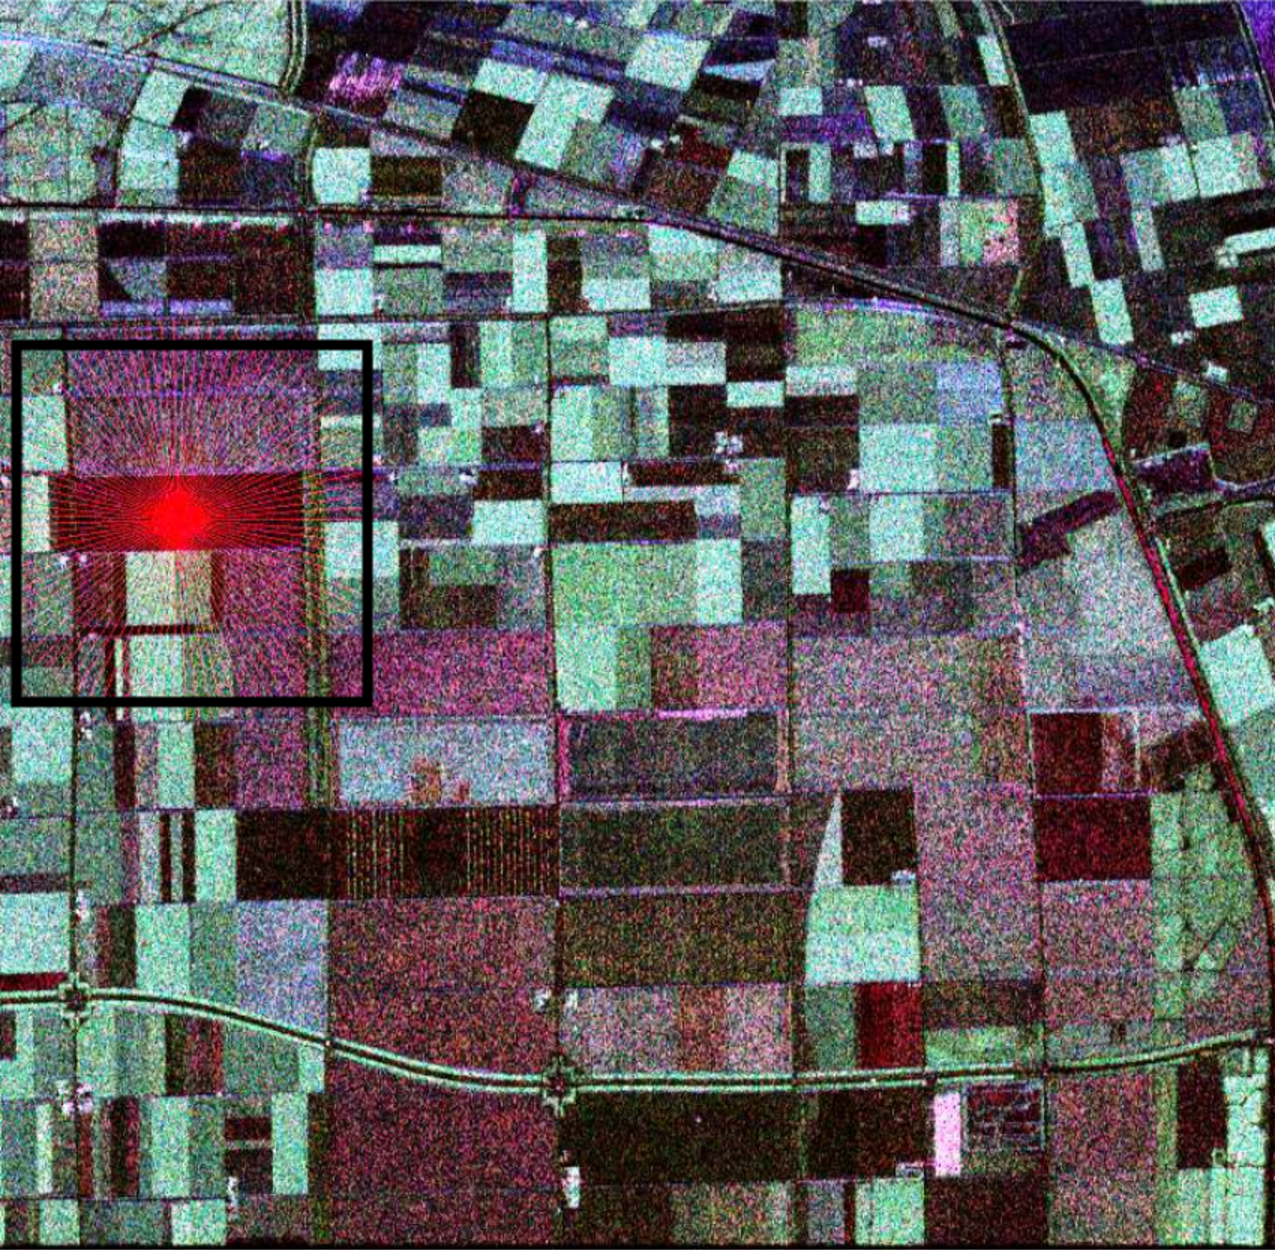
\includegraphics[width=.5\linewidth]{flevoland_radial_4_look_black}
	\caption{Region of interest (ROI) in the image of Flevoland.}
\label{fig10}
\end{figure}
\end{alertblock}
\end{frame}


\begin{frame}[fragile]{Results}
\begin{alertblock}{Results}
	\begin{figure}[hbt]
	\centering
     \subfloat[Evidences in channel $\text{hh}$ \label{evidencias_hh_hv_vv:a}]{%
     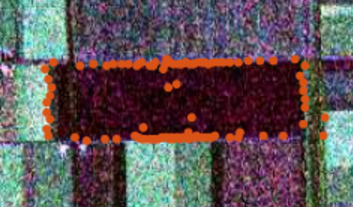
\includegraphics[width=0.45\textwidth]{flevoland_100_point_hh_crop}              
      % 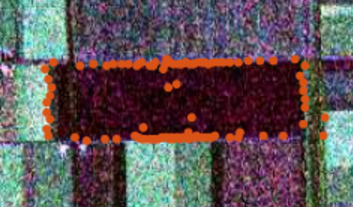
\includegraphics[viewport= 100 0 490 460, clip=true, width=0.3\linewidth]               {flevoland_100_point_hh_crop}
     }\qquad
     \subfloat[Evidences in channel $\text{hv}$ \label{evidencias_hh_hv_vv:b}]{%
       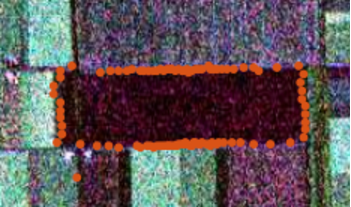
\includegraphics[width=0.45\linewidth]{flevoland_100_point_hv_crop}
     }\qquad
     \subfloat[Evidences in channel $\text{vv}$ \label{evidencias_hh_hv_vv:c}]{%
       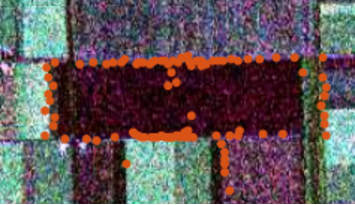
\includegraphics[width=0.45\linewidth]{flevoland_100_point_vv_crop}
     }
    \caption{Evidence by channel}
     \label{fig11}
   \end{figure}	
\end{alertblock}
\end{frame}

\begin{frame}[fragile]{Results}
	\begin{figure}[hbt]
	\centering
     \subfloat[Average Fusion \label{evidencias_hh_hv_vv:a}]{%
       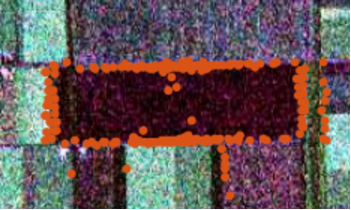
\includegraphics[width=0.45\linewidth]{flevoland_100_media_crop}
     }\quad
     \subfloat[PCA Fusion\label{evidencias_hh_hv_vv:b}]{%
       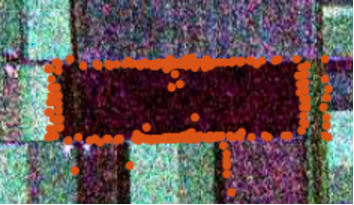
\includegraphics[width=0.45\linewidth]{flevoland_100_pca_crop}
     }\\
     \subfloat[DWT Fusion \label{evidencias_hh_hv_vv:a}]{%
       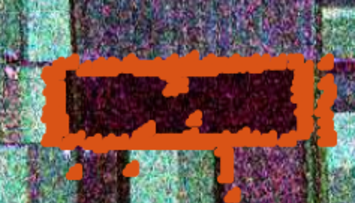
\includegraphics[width=0.45\linewidth]{flevoland_100_dwt_crop}
     }\quad
     \subfloat[SWT Fusion \label{evidencias_hh_hv_vv:c}]{%
       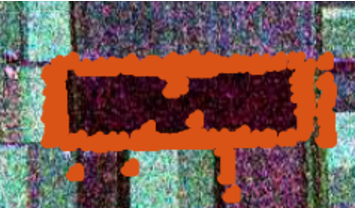
\includegraphics[width=0.45\linewidth]{flevoland_100_swt_crop}
     }
     \caption{Evidence after fusion}
     \label{fig12}
   \end{figure}	
\end{frame}
\begin{frame}[fragile]{Results}
	\begin{figure}[hbt]
	\centering
     \subfloat[ROC Fusion \label{evidencias_hh_hv_vv:a}]{%
       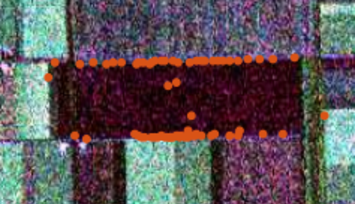
\includegraphics[width=0.45\linewidth]{flevoland_100_roc_crop}
     }\quad
     \subfloat[SVD Fusion\label{evidencias_hh_hv_vv:b}]{%
       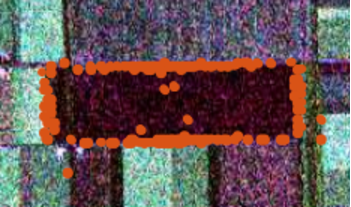
\includegraphics[width=0.45\linewidth]{flevoland_100_svd_crop}
     }
     \caption{Evidence after fusion}
     \label{fig12}
   \end{figure}	
\end{frame}

\begin{frame}[fragile]{Conclusion}
\begin{alertblock}{Conclusion}
\begin{itemize}
	\item Simulated Annealing works very well in non differentiable function. Figure~(\ref{fig4}) shows the probability of detecting edges evidences;
	\item The method to detect edges evidence in each channel works very well. See Figure~(\ref{fig11}). Similar ideas can be found in  Refs.~\cite{fbgm,nhfc};
	\item The fusion of evidence in intensity channels shows that these channels can be complementary and, therefore, suitable for edge detection in PolSAR images. See Figure~(\ref{fig12}).
	\item The article shows the viability of these methods and your extension to more channels.
\end{itemize}
\end{alertblock}
\begin{alertblock}{Future researches}	
\begin{itemize}
	\item Increase the number of channels to improve the fusion;
	\item Investigate new fusion methods.
\end{itemize}
\end{alertblock}
\end{frame}

\begin{frame}[allowframebreaks]
\bibliographystyle{IEEEtran}
\bibliography{../bibliografia}
\end{frame}
\end{document}
